% Build: cd docs/lightning_talk && latexmk -pdf lightning_talk.tex
% Lightning talk for 18-660/18-460 (Spring 2026), 5-minute strict limit.
\documentclass[aspectratio=169,11pt]{beamer}

\usetheme{default}
\usecolortheme{dolphin}
\setbeamertemplate{navigation symbols}{}
\setbeamertemplate{footline}[frame number]
\setbeamerfont{frametitle}{size=\large,series=\bfseries}

\usepackage{graphicx}
\usepackage{booktabs}
\usepackage{amsmath}
\usepackage{array}

\graphicspath{{figures/}}

\newcommand{\dmin}{d_{\min}}
\newcommand{\bad}[1]{\textcolor{red!70!black}{\textbf{#1}}}
\newcommand{\good}[1]{\textcolor{green!45!black}{\textbf{#1}}}

\title[ADMM vs.\ Penalty for Multi-Drone MPC]{%
  Comparing ADMM and Penalty Methods for\\
  Distributed Multi-Agent Trajectory Planning}
\author{Christian Yu \and Yuyang Wu \and Yen-Ru Chin}
\institute{Department of Electrical and Computer Engineering\\Carnegie Mellon University}
\date{18-660 / 18-460 Lightning Talk \\ April 23, 2026}

\begin{document}

% --- Slide 1: Title -----------------------------------------------------
\begin{frame}
  \titlepage
\end{frame}

% --- Slide 2: Background / Motivation ------------------------------------
\begin{frame}{Background \& Motivation}
  \begin{columns}[T,onlytextwidth]
    \begin{column}{0.58\textwidth}
      \begin{itemize}
        \item \textbf{Problem.} $N$ drones must reach individual goals
              while avoiding collisions\,---\,but no central coordinator
              sees all states.
        \item \textbf{Per-agent MPC} (convex QP after linearizing
              $\|p_i - p_j\| \ge \dmin$ at each step):
              \[
                \min_{x_i,u_i}\!\!\sum_{k=0}^{H-1}\!
                \bigl(\|x_i(k)\!-\!x_i^{\text{ref}}(k)\|_Q^2
                     +\|u_i(k)\|_R^2\bigr)
              \]
        \item \textbf{Two distributed paradigms} differ in how they
              handle the \emph{coupling} between agents:
              \begin{itemize}
                \item \emph{Penalty:} soft cost on violation.
                \item \emph{Consensus ADMM:} dual-variable feedback
                      drives feasibility in the limit.
              \end{itemize}
      \end{itemize}
    \end{column}
    \begin{column}{0.42\textwidth}
      \small
      \textbf{Why it matters.}\\[0.3em]
      Cyber-physical systems\,---\,delivery swarms, robot fleets,
      multi-vehicle coordination\,---\,need distributed optimizers
      that are both
      \good{feasible} (no collisions) and
      \good{tractable} (per-agent QPs at each round).
    \end{column}
  \end{columns}
\end{frame}

% --- Slide 3: Key Question ----------------------------------------------
\begin{frame}{Key Question}
  \begin{center}
    \Large
    \emph{Does ADMM's dual-variable machinery earn its extra complexity\\
    over a simple distributed penalty baseline\\
    on multi-drone trajectory planning?}
  \end{center}
  \vspace{1em}
  \begin{itemize}
    \item Do both methods reach the \textbf{centralized optimum}?
    \item How sensitive is each to its tuning knob\,---\,$w$ for penalty, $\rho$ for ADMM?
    \item Does the comparison hold as we \textbf{scale} from $N{=}4$ to $N{=}8$?
  \end{itemize}
\end{frame}

% --- Slide 4: Take-home 1 -----------------------------------------------
\begin{frame}{Take-home 1: All three reach goals; only penalty collides}
  \begin{center}
    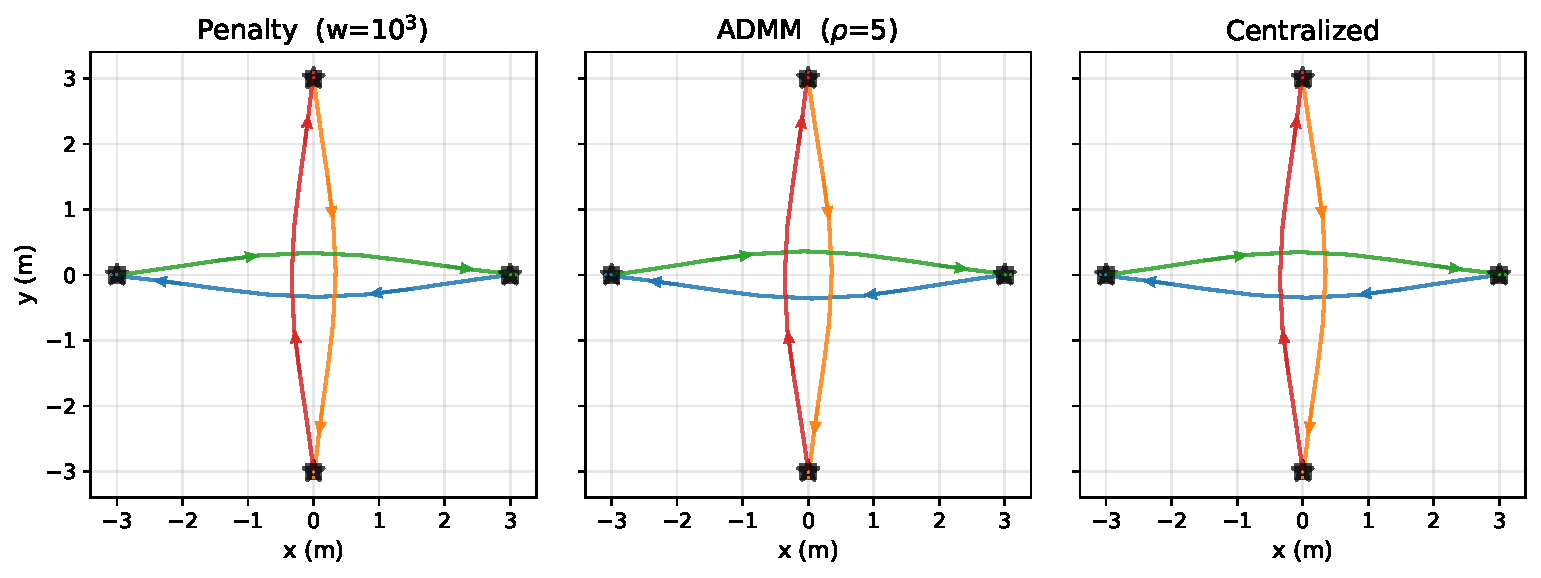
\includegraphics[width=0.92\linewidth]{fig_s2_trajectories.pdf}
  \end{center}
  \vspace{-0.7em}
  \begin{center}\footnotesize
    \begin{tabular}{@{}lcccc@{}}
      \toprule
      S2 ($N{=}4$, ring graph) & iters & $J^\star$ & min-dist (m) & violation (m) \\
      \midrule
      Penalty ($w{=}10^3$)         & 99 & 8944.8 & \bad{0.483}  & \bad{$1.67{\times}10^{-2}$} \\
      ADMM ($\rho{=}5$)            & 44 & 8948.6 & \good{0.517} & \good{$0$} \\
      Centralized                  & 5  & 8946.5 & 0.500        & $0$ \\
      \bottomrule
    \end{tabular}
  \end{center}
  \vspace{0.2em}
  \begin{itemize}
    \footnotesize
    \item All three objectives agree within $0.04\%$, but penalty's
          \bad{min-distance $0.483\,\text{m} < \dmin{=}0.5$}\,---\,a real
          collision hidden by soft slack.
  \end{itemize}
\end{frame}

% --- Slide 5: Take-home 2 -----------------------------------------------
\begin{frame}{Take-home 2: Penalty has a U-shape in $w$; ADMM doesn't}
  \begin{center}
    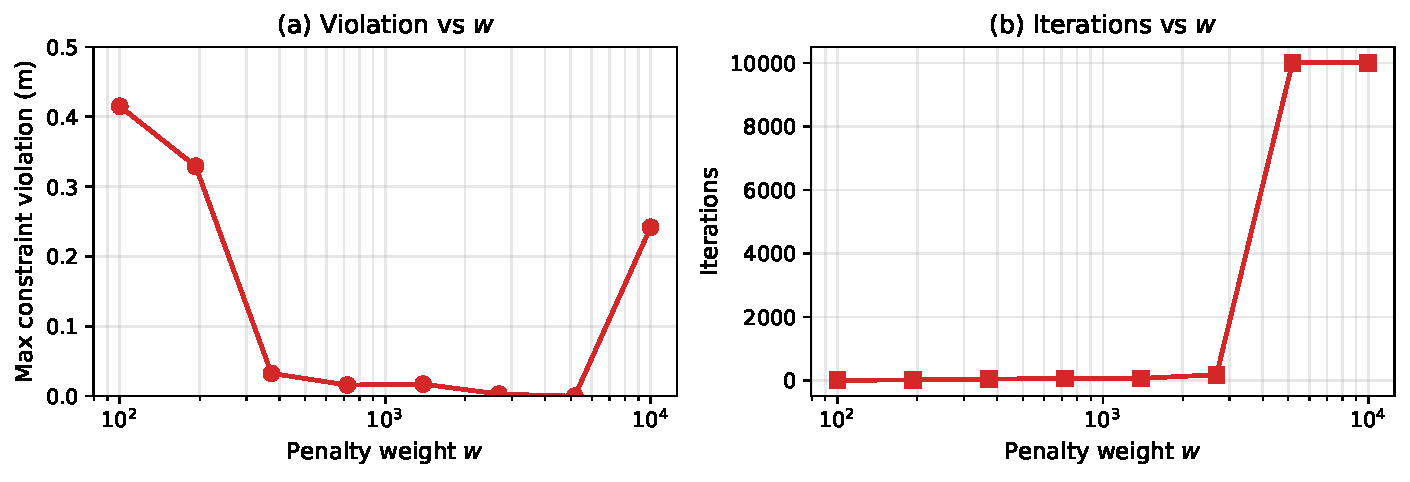
\includegraphics[width=0.96\linewidth]{fig_w_sensitivity.pdf}
  \end{center}
  \vspace{-0.6em}
  \begin{itemize}
    \footnotesize
    \item \bad{Small $w$:} collision cost too weak\,---\,drones overlap
          by up to $0.42$\,m.
          \bad{Large $w$:} collision cost dominates the QP; the solver
          can't converge in 500 iterations and still leaves $0.24$\,m
          of overlap.
    \item \textbf{Why ADMM has no such knob:}
          the scaled dual update
          $\lambda_{ij}\!\leftarrow\!\lambda_{ij}\!+\!\rho(\theta_i\!-\!\theta_j)$
          integrates consensus errors iteratively, decoupling
          feasibility-driving from QP conditioning.
  \end{itemize}
\end{frame}

% --- Slide 6: Take-home 3 -----------------------------------------------
\begin{frame}{Take-home 3: Gap widens at $N{=}8$}
  \begin{center}
    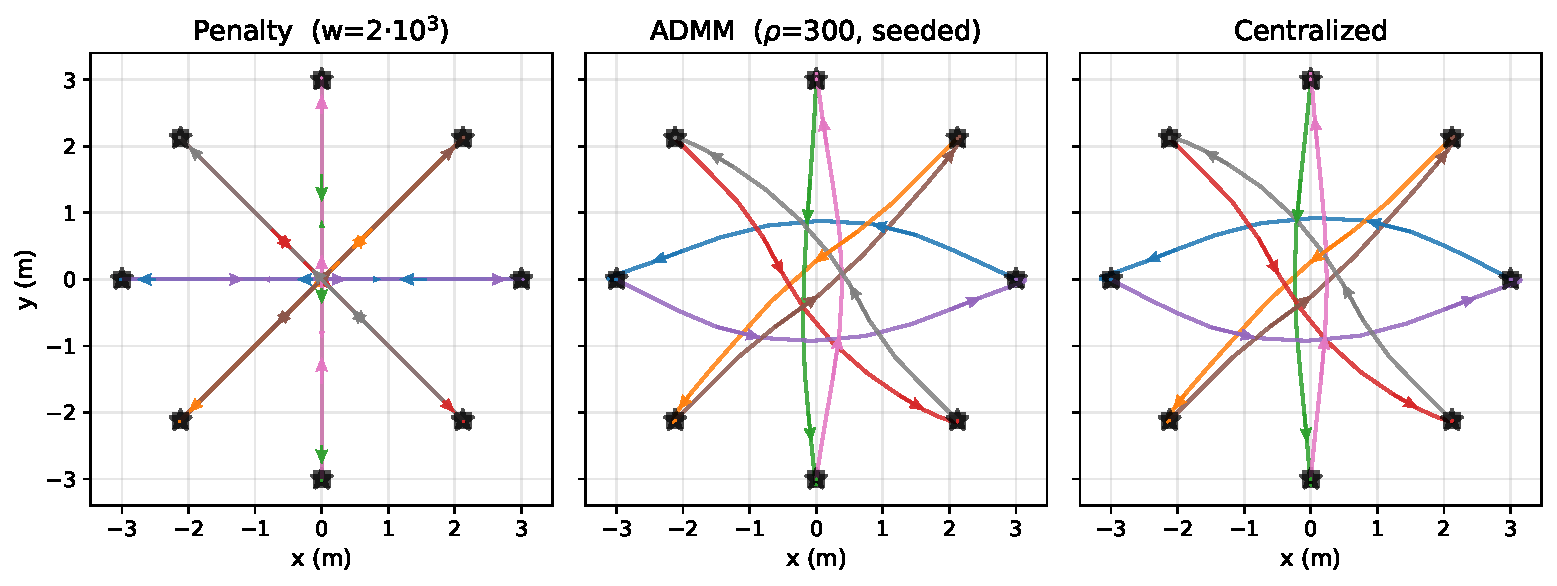
\includegraphics[width=0.95\linewidth]{fig_s3_trajectories.pdf}
  \end{center}
  \vspace{-0.8em}
  \begin{center}\footnotesize
    \begin{tabular}{@{}lcccc@{}}
      \toprule
      S3 ($N{=}8$, complete graph) & iters & $J^\star$ & min-dist (m) & violation (m) \\
      \midrule
      Penalty ($w{=}2{\cdot}10^3$) & 20  & \bad{26981}  & \bad{0.175}  & \bad{$3.25{\times}10^{-1}$} \\
      ADMM ($\rho{=}300$, seeded)  & 111 & \good{17125} & \good{0.500} & \good{$1.2{\times}10^{-4}$} \\
      Centralized                  & 5   & 17120        & 0.500        & $\approx 0$ \\
      \bottomrule
    \end{tabular}
  \end{center}
  \vspace{0.2em}
  \begin{itemize}
    \footnotesize
    \item ADMM matches centralized to \good{$0.03\%$ on $J^\star$};
          penalty's drones overlap by \bad{$0.33\,\text{m}$}\,---\,the
          feasibility gap grew \bad{${\sim}20{\times}$} from S2 to S3.
  \end{itemize}
\end{frame}

% --- Slide 7: Summary ---------------------------------------------------
\begin{frame}{When to use which\,---\,and why ADMM's duals matter}
  \begin{center}\small
    \begin{tabular}{@{}lccc@{}}
      \toprule
                                 & \textbf{Penalty} & \textbf{ADMM}       & \textbf{Centralized} \\
      \midrule
      Implementation complexity  & low              & medium              & low \\
      Per-iteration cost         & $N$ small QPs    & $N$ larger QPs      & 1 joint QP \\
      Feasibility guarantee      & none ($w$-dep.)  & in the limit        & hard \\
      Tuning knobs               & $w$              & $\rho$              & solver only \\
      Work per iteration         & $\mathcal{O}(N)$ parallel & $\mathcal{O}(N)$ parallel & $\mathcal{O}(N^2)$ central \\
      \bottomrule
    \end{tabular}
  \end{center}
  \vspace{0.8em}
  \begin{center}
    \textbf{Thesis.} ADMM's dual-variable feedback pays off exactly where
    penalty's single $w$ knob runs out of room\,---\,the gap grows with
    the number of coupled agents.
  \end{center}
\end{frame}

% --- Slide 8 (optional backup): Acknowledgements ------------------------
\begin{frame}{Thank you}
  \begin{itemize}
    \item Code, configs, and animated comparison videos:\\
          \texttt{github.com/chrisjinyu/distributed-trajectory-planning}
    \item \textbf{Selected references.}
          \begin{itemize}\footnotesize
            \item Boyd, Parikh, Chu, Peleato \& Eckstein (2011).\\
                  \emph{Distributed Optimization and Statistical
                  Learning via ADMM.}
            \item Chen (2024). \emph{A brief tutorial on consensus ADMM
                  for distributed optimization with applications in
                  robotics.}
          \end{itemize}
  \end{itemize}
  \vspace{1.0em}
  \begin{center}
    \Large Questions?
  \end{center}
\end{frame}

\end{document}
